% !TEX TS-program = pdflatex
%
% File acl2017.tex
%
%% Based on the style files for ACL-2015, with some improvements
%%  taken from the NAACL-2016 style
%% Based on the style files for ACL-2014, which were, in turn,
%% based on ACL-2013, ACL-2012, ACL-2011, ACL-2010, ACL-IJCNLP-2009,
%% EACL-2009, IJCNLP-2008...
%% Based on the style files for EACL 2006 by 
%%e.agirre@ehu.es or Sergi.Balari@uab.es
%% and that of ACL 08 by Joakim Nivre and Noah Smith

\documentclass[11pt,a4paper]{article}
\usepackage[hyperref]{acl2017}
\usepackage{times}
\usepackage{latexsym}
\usepackage{graphicx}
\graphicspath{ {pictures/} }
\usepackage{url}
\usepackage{amsmath}

\aclfinalcopy % Uncomment this line for the final submission
%\def\aclpaperid{***} %  Enter the acl Paper ID here

%\setlength\titlebox{5cm}
% You can expand the titlebox if you need extra space
% to show all the authors. Please do not make the titlebox
% smaller than 5cm (the original size); we will check this
% in the camera-ready version and ask you to change it back.

\newcommand\BibTeX{B{\sc ib}\TeX}

\title{Instructions for ACL-2017 Proceedings}

\author{Haonan Li \\
  {\tt email@domain} \\\And
  Keyong Huang \\
  {\tt email@domain} \\\And
    Keyong Huang \\
  {\tt email@domain} \\\
 }

\date{6.29.2017}

\begin{document}

\maketitle
\begin{abstract}
Latent Dirichlet Allocation(LDA) is a popular algorithm for Topic Modelling, which is widely used in many fields like e-commerce, document summarised, etc. In this project, we're trying to realise the LDA via Gibbs Sampling in python and then conduct empirical analysis on three different tasks - document modelling, document classification and collaborative filtering(CF). And our results show LDA performs well in document modelling and CF, but unsatisfactory in document classification.
\end{abstract}

\section{Introduction}

The goal of topic modeling is to discern latent topics of a collection of documents. To specify, the project requires us to find the topic structures of the corpus according to the content based on the statistical relationship between them, which is useful in numerous tasks. LDA is a generative model based on the simple 'bag-of-words' assumption. The variations of LDA also raise a lot of attention in recent years. However, we will limit our passage only to the traditional LDA method and its applicaitions.   

The paper is organised as follows. In Section 2 we will introduce the basic idea of Latent Dirichlet Allocation(LDA) via Gibbs Sampling and how we implement it in Python. In Section 3, we will focus on the task of topic modeling. We will introduce the document classification in Section 4. In Section 5, we will present you with empirical result in collaborative filtering. 


%\section{Data Preprocessing}
%As the convention of natural language preprocessing, we remove stopwords 
%like 'we','us' in all documents and stem them afterwards. In order to make 

\section{Introduction and Implementation of LDA}

Latent Dirichlet Allocation(LDA) is a hierarchical model for topic modelling. Unlike simple algorithms like PLSI, LDA assume that a single document may comprise of several different topics.The graphical representation is as Figure1.The detailed explanation of LDA model can be found in Ng, Blei(2013).

\begin{figure}[h]
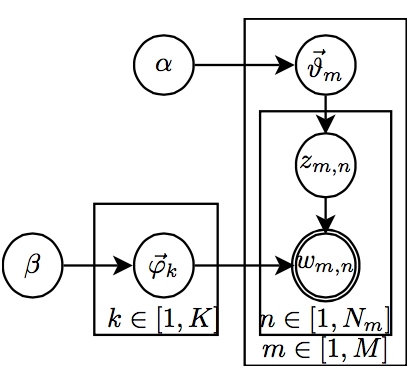
\includegraphics[scale=0.8]{graphic_rep.png}
\centering
\caption{Graphical Representation of LDA}
\centering
\end{figure}

The inference of posterior distribution can be considered in different ways. In this article, we will use Gibbs Sampling to implement LDA. The Gibbs Sampling is a popular Monte Carlo sampling method. The essence of this method is to compute the conditional distrition $P(z_i | x, z^{\neg}_i ) $, where $z^{\neg}_i$ indicates all z except $z_i$ for token i. After calculation, we have:

\begin{displaymath}
P(z_i | x, z^{\neg}_i ) \propto \frac{n^{t}_{k, \neg i} + \beta}{ \sum_{t=1}^{V} n^{t}_{k, \neg i}+ V\beta}
\frac{n^{k}_{m, \neg i} + \alpha}{ \sum_{k=1}^{V} n^{k}_{m}+ K\alpha}
\end{displaymath}

where $n^{t}_{k, \neg i}$ means the number of tokens assigned to topic k excluding token i, $n^{k}_{m, \neg i}$  indicates the number of tokens assign to topic k in document m excluding token i, corresponding to topic-term matrix and document-topic matrix.

Meanwhile, the number of iteration of Gibbs Sampling should be carefully assigned to speed up the whole process. In hindsight, 500 is an optimal number for the stationary sampling.

Afterwards, we need computer two values of interest: the term distribution for each topic and the topic distribution for each document, namely $\theta_m$ and $\phi_k$, where m=
$1,2, \dots, M$ and k = $1,2,\dots, K$. The result is as following:

\begin{displaymath}
\phi_{k,t}= \frac{n^{t}_{k} + \beta}{ \sum_{t=1}^{V} n^{t}_{k}+ V\beta}
\end{displaymath}
\begin{displaymath}
\theta_{m,k} =  \frac{n^{k}_{m} + \alpha}{ \sum_{k=1}^{K} n^{k}_{m}+ K\alpha}
\end{displaymath}

In terms of the parameter tuning, common criterion is the perplexity of the test datasets. However, due to the goal of the specific task, one may find some changes on the
metric of perplexity more appropriate. Thus, we will introduce this metric in detail later when we introduce the tasks.

\section{Document Modelling}

In order to figure out the most suitable number of topics according to the content and semanteme based on the statistical features, we need a large set of data to train the data. Furthermore, we ensured the accuracy of the algorithm by comparing with other graphic modeling algorithm.


Reviewers: note that the ruler measurements do not align well with
lines in the paper -- this turns out to be very difficult to do well
when the paper contains many figures and equations, and, when done,
looks ugly. In most cases one would expect that the approximate
location will be adequate, although you can also use fractional
references ({\em e.g.}, the first paragraph on this page ends at mark $114.5$).

\subsection{Data description}

The dataset we use is Amazon Fine Foods reviews, which consists of 568,454 reviews of fine foods from 256,059 users left up to Oct. 2012. 
Amazon fine food reviews dataset has the following attributes: ProductId, UserId�, ProfileName, HelpfulnessNumerator (number of users who found the review helpful),  HelpfulnessDenominator (number of users who indicated whether they found the review helpful)�, Score (rating of the product), Time�, Summary(brief summary of the review)� and Text(text of the review).

In our document classification problem, we use text information, Summary and Text as the corpus to train and test the LDA model. Score, whose rating between one and five, is the categorical variable in the document classification model. By applying LDA model, we can use a dense document-topic matrix derived by LDA model to replace a sparse co-occurrence matrix, thus serving a function of dimensionality reduction.

However the original dataset is too large thus too time-consuming for us to train the LDA model, so we randomly choose 1500 reviews from 1478 users evaluating 1318 products.

\subsection{Choose appropriate number of topics}
\label{sect:pdf}

For the production of the electronic manuscript you must use Adobe's
Portable Document Format (PDF). PDF files are usually produced from
\LaTeX\ using the \textit{pdflatex} command. If your version of
\LaTeX\ produces Postscript files, you can convert these into PDF
using \textit{ps2pdf} or \textit{dvipdf}. On Windows, you can also use
Adobe Distiller to generate PDF.

Please make sure that your PDF file includes all the necessary fonts
(especially tree diagrams, symbols, and fonts with Asian
characters). When you print or create the PDF file, there is usually
an option in your printer setup to include none, all or just
non-standard fonts.  Please make sure that you select the option of
including ALL the fonts. \textbf{Before sending it, test your PDF by
  printing it from a computer different from the one where it was
  created.} Moreover, some word processors may generate very large PDF
files, where each page is rendered as an image. Such images may
reproduce poorly. In this case, try alternative ways to obtain the
PDF. One way on some systems is to install a driver for a postscript
printer, send your document to the printer specifying ``Output to a
file'', then convert the file to PDF.

It is of utmost importance to specify the \textbf{A4 format} (21 cm
x 29.7 cm) when formatting the paper. When working with
{\tt dvips}, for instance, one should specify {\tt -t a4}.
Or using the command \verb|\special{papersize=210mm,297mm}| in the latex
preamble (directly below the \verb|\usepackage| commands). Then using 
{\tt dvipdf} and/or {\tt pdflatex} which would make it easier for some.

Print-outs of the PDF file on A4 paper should be identical to the
hardcopy version. If you cannot meet the above requirements about the
production of your electronic submission, please contact the
publication chairs as soon as possible.

\subsection{Layout}
\label{ssec:layout}

Format manuscripts two columns to a page, in the manner these
instructions are formatted. The exact dimensions for a page on A4
paper are:

\begin{itemize}
\item Left and right margins: 2.5 cm
\item Top margin: 2.5 cm
\item Bottom margin: 2.5 cm
\item Column width: 7.7 cm
\item Column height: 24.7 cm
\item Gap between columns: 0.6 cm
\end{itemize}

\noindent Papers should not be submitted on any other paper size.
 If you cannot meet the above requirements about the production of 
 your electronic submission, please contact the publication chairs 
 above as soon as possible.

\subsection{Fonts}

For reasons of uniformity, Adobe's {\bf Times Roman} font should be
used. In \LaTeX2e{} this is accomplished by putting

\begin{quote}
\begin{verbatim}
\usepackage{times}
\usepackage{latexsym}
\end{verbatim}
\end{quote}
in the preamble. If Times Roman is unavailable, use {\bf Computer
  Modern Roman} (\LaTeX2e{}'s default).  Note that the latter is about
  10\% less dense than Adobe's Times Roman font.

\begin{table}[h]
\begin{center}
\begin{tabular}{|l|rl|}
\hline \bf Type of Text & \bf Font Size & \bf Style \\ \hline
paper title & 15 pt & bold \\
author names & 12 pt & bold \\
author affiliation & 12 pt & \\
the word ``Abstract'' & 12 pt & bold \\
section titles & 12 pt & bold \\
document text & 11 pt  &\\
captions & 11 pt & \\
abstract text & 10 pt & \\
bibliography & 10 pt & \\
footnotes & 9 pt & \\
\hline
\end{tabular}
\end{center}
\caption{\label{font-table} Font guide. }
\end{table}

\subsection{The First Page}
\label{ssec:first}

Center the title, author's name(s) and affiliation(s) across both
columns. Do not use footnotes for affiliations. Do not include the
paper ID number assigned during the submission process. Use the
two-column format only when you begin the abstract.

{\bf Title}: Place the title centered at the top of the first page, in
a 15-point bold font. (For a complete guide to font sizes and styles,
see Table~\ref{font-table}) Long titles should be typed on two lines
without a blank line intervening. Approximately, put the title at 2.5
cm from the top of the page, followed by a blank line, then the
author's names(s), and the affiliation on the following line. Do not
use only initials for given names (middle initials are allowed). Do
not format surnames in all capitals ({\em e.g.}, use ``Mitchell'' not
``MITCHELL'').  Do not format title and section headings in all
capitals as well except for proper names (such as ``BLEU'') that are
conventionally in all capitals.  The affiliation should contain the
author's complete address, and if possible, an electronic mail
address. Start the body of the first page 7.5 cm from the top of the
page.

The title, author names and addresses should be completely identical
to those entered to the electronical paper submission website in order
to maintain the consistency of author information among all
publications of the conference. If they are different, the publication
chairs may resolve the difference without consulting with you; so it
is in your own interest to double-check that the information is
consistent.

{\bf Abstract}: Type the abstract at the beginning of the first
column. The width of the abstract text should be smaller than the
width of the columns for the text in the body of the paper by about
0.6 cm on each side. Center the word {\bf Abstract} in a 12 point bold
font above the body of the abstract. The abstract should be a concise
summary of the general thesis and conclusions of the paper. It should
be no longer than 200 words. The abstract text should be in 10 point font.

{\bf Text}: Begin typing the main body of the text immediately after
the abstract, observing the two-column format as shown in 
the present document. Do not include page numbers.

{\bf Indent}: When starting a new paragraph. Use 11 points for text and 
subsection headings, 12 points for section headings and 15 points for
the title. 

\begin{table}
\centering
\small
\begin{tabular}{cc}
\begin{tabular}{|l|l|}
\hline
{\bf Command} & {\bf Output}\\\hline
\verb|{\"a}| & {\"a} \\
\verb|{\^e}| & {\^e} \\
\verb|{\`i}| & {\`i} \\ 
\verb|{\.I}| & {\.I} \\ 
\verb|{\o}| & {\o} \\
\verb|{\'u}| & {\'u}  \\ 
\verb|{\aa}| & {\aa}  \\\hline
\end{tabular} & 
\begin{tabular}{|l|l|}
\hline
{\bf Command} & {\bf  Output}\\\hline
\verb|{\c c}| & {\c c} \\ 
\verb|{\u g}| & {\u g} \\ 
\verb|{\l}| & {\l} \\ 
\verb|{\~n}| & {\~n} \\ 
\verb|{\H o}| & {\H o} \\ 
\verb|{\v r}| & {\v r} \\ 
\verb|{\ss}| & {\ss} \\\hline
\end{tabular}
\end{tabular}
\caption{Example commands for accented characters, to be used in, {\em e.g.}, \BibTeX\ names.}\label{tab:accents}
\end{table}

\subsection{Sections}

{\bf Headings}: Type and label section and subsection headings in the
style shown on the present document.  Use numbered sections (Arabic
numerals) in order to facilitate cross references. Number subsections
with the section number and the subsection number separated by a dot,
in Arabic numerals. Do not number subsubsections.

\begin{table*}
\centering
\begin{tabular}{lll}
  output & natbib & previous ACL style files\\
  \hline
  \citep{Gusfield:97} & \verb|\citep| & \verb|\cite| \\
  \citet{Gusfield:97} & \verb|\citet| & \verb|\newcite| \\
  \citeyearpar{Gusfield:97} & \verb|\citeyearpar| & \verb|\shortcite| \\
\end{tabular}
\caption{Citation commands supported by the style file.
  The citation style is based on the natbib package and
  supports all natbib citation commands.
  It also supports commands defined in previous ACL style files
  for compatibility.
  }
\end{table*}

{\bf Citations}: Citations within the text appear in parentheses
as~\cite{Gusfield:97} or, if the author's name appears in the text
itself, as Gusfield~\shortcite{Gusfield:97}.
Using the provided \LaTeX\ style, the former is accomplished using
{\small\verb|\cite|} and the latter with {\small\verb|\shortcite|} or {\small\verb|\newcite|}.  Collapse multiple citations as in~\cite{Gusfield:97,Aho:72}; this is accomplished with the provided style using commas within the {\small\verb|\cite|} command, {\em e.g.}, {\small\verb|\cite{Gusfield:97,Aho:72}|}.  
Append lowercase letters to the year in cases of ambiguities.  
 Treat double authors as
in~\cite{Aho:72}, but write as in~\cite{Chandra:81} when more than two
authors are involved. Collapse multiple citations as
in~\cite{Gusfield:97,Aho:72}. Also refrain from using full citations
as sentence constituents.

\penalty -5000

We suggest that instead of
\begin{quote}
  ``\cite{Gusfield:97} showed that ...''
\end{quote}
you use
\begin{quote}
``Gusfield \shortcite{Gusfield:97}   showed that ...''
\end{quote}

If you are using the provided \LaTeX{} and Bib\TeX{} style files, you
can use the command \verb|\citet| (cite in text)
to get ``author (year)'' citations.

If the Bib\TeX{} file contains DOI fields, the paper
title in the references section will appear as a hyperlink
to the DOI, using the hyperref \LaTeX{} package.
To disable the hyperref package, load the style file
with the \verb|nohyperref| option:
\verb|\usepackage[nohyperref]{acl2017}|

\textbf{Digital Object Identifiers}:  As part of our work to make ACL
materials more widely used and cited outside of our discipline, ACL
has registered as a CrossRef member, as a registrant of Digital Object
Identifiers (DOIs), the standard for registering permanent URNs for
referencing scholarly materials.  As of 2017, we are requiring all
camera-ready references to contain the appropriate DOIs (or as a
second resort, the hyperlinked ACL Anthology Identifier) to all cited
works.  Thus, please ensure that you use Bib\TeX records that contain
DOI or URLs for any of the ACL materials that you reference.
Appropriate records should be found for most materials in the current
ACL Anthology at \url{http://aclanthology.info/}.

As examples, we cite \cite{P16-1001} to show you how papers with a DOI
will appear in the bibliography.  We cite \cite{C14-1001} to show how
papers without a DOI but with an ACL Anthology Identifier will appear
in the bibliography.  

As reviewing will be double-blind, the submitted version of the papers
should not include the authors' names and affiliations. Furthermore,
self-references that reveal the author's identity, {\em e.g.},
\begin{quote}
``We previously showed \cite{Gusfield:97} ...''  
\end{quote}
should be avoided. Instead, use citations such as 
\begin{quote}
``\citeauthor{Gusfield:97} \shortcite{Gusfield:97}
previously showed ... ''
\end{quote}

\textbf{Please do not use anonymous citations} and do not include
acknowledgements when submitting your papers. Papers that do not
conform to these requirements may be rejected without review.

\textbf{References}: Gather the full set of references together under
the heading {\bf References}; place the section before any Appendices,
unless they contain references. Arrange the references alphabetically
by first author, rather than by order of occurrence in the text.
Provide as complete a citation as possible, using a consistent format,
such as the one for {\em Computational Linguistics\/} or the one in the 
{\em Publication Manual of the American 
Psychological Association\/}~\cite{APA:83}.  Use of full names for
authors rather than initials is preferred.  A list of abbreviations
for common computer science journals can be found in the ACM 
{\em Computing Reviews\/}~\cite{ACM:83}.

The \LaTeX{} and Bib\TeX{} style files provided roughly fit the
American Psychological Association format, allowing regular citations, 
short citations and multiple citations as described above.

{\bf Appendices}: Appendices, if any, directly follow the text and the
references (but see above).  Letter them in sequence and provide an
informative title: {\bf Appendix A. Title of Appendix}.

\subsection{Footnotes}

{\bf Footnotes}: Put footnotes at the bottom of the page and use 9
points text. They may be numbered or referred to by asterisks or other
symbols.\footnote{This is how a footnote should appear.} Footnotes
should be separated from the text by a line.\footnote{Note the line
separating the footnotes from the text.}

\subsection{Graphics}

{\bf Illustrations}: Place figures, tables, and photographs in the
paper near where they are first discussed, rather than at the end, if
possible.  Wide illustrations may run across both columns.  Color
illustrations are discouraged, unless you have verified that  
they will be understandable when printed in black ink.

{\bf Captions}: Provide a caption for every illustration; number each one
sequentially in the form:  ``Figure 1. Caption of the Figure.'' ``Table 1.
Caption of the Table.''  Type the captions of the figures and 
tables below the body, using 11 point text.

\subsection{Accessibility}
\label{ssec:accessibility}

In an effort to accommodate the color-blind (as well as those printing
to paper), grayscale readability for all accepted papers will be
encouraged.  Color is not forbidden, but authors should ensure that
tables and figures do not rely solely on color to convey critical
distinctions.
Here we give a simple criterion on your colored figures, if your paper has to be printed in black and white, then you must assure that every curves or points in your figures can be still clearly distinguished.

% Min: no longer used as of ACL 2017, following ACL exec's decision to
% remove this extra workflow that was not executed much.
% BEGIN: remove
%% \section{XML conversion and supported \LaTeX\ packages}

%% Following ACL 2014 we will also we will attempt to automatically convert 
%% your \LaTeX\ source files to publish papers in machine-readable 
%% XML with semantic markup in the ACL Anthology, in addition to the 
%% traditional PDF format.  This will allow us to create, over the next 
%% few years, a growing corpus of scientific text for our own future research, 
%% and picks up on recent initiatives on converting ACL papers from earlier 
%% years to XML. 

%% We encourage you to submit a ZIP file of your \LaTeX\ sources along
%% with the camera-ready version of your paper. We will then convert them
%% to XML automatically, using the LaTeXML tool
%% (\url{http://dlmf.nist.gov/LaTeXML}). LaTeXML has \emph{bindings} for
%% a number of \LaTeX\ packages, including the ACL 2017 stylefile. These
%% bindings allow LaTeXML to render the commands from these packages
%% correctly in XML. For best results, we encourage you to use the
%% packages that are officially supported by LaTeXML, listed at
%% \url{http://dlmf.nist.gov/LaTeXML/manual/included.bindings}
% END: remove

\section{Collaborative Filtering}

In our task of Collaborative Filtering(CF), we conduct LDA algorithm on the dataset from platform for movie reviewers ? MovieLens, to predict the preference of users and recommend them a new movie based on the their records. The dataset we are using is MoiveLens 20M(2016) and only a subset of it(2000 users in 138000) is included in our experiment due to the lack of computational resources. 

In our experiment, all users having less than 100 reviews are not included into our dataset in order to partly control the problem of sparsity. We divide this set of users into 1800 training users and 200 testing users. Training users will be further divided for the parameter tuning, which is number of topics in the LDA model. We train the model on a fully observed set of users. For each user in the test dataset, we hold out one movie in their records and use the others to guess the held-out movie. The evaluation metric is the likelihood of the held-out movie. More precisely, we define the predictive-perplexity as following:

\begin{small}
\begin{displaymath}
P\textrm{-}P(D_{test}) =  
 \exp{\left\{-\frac{\sum_{d=1}^M \log p(w_{d,N_d}|\mathbf{w}_{d,1:N_d-1})}{M}\right\}}
\end{displaymath}
\end{small}
\subsection{Model Training}

We split the training dataset into two groups, 80\% for modeling and 20\% for parameter tuning. And then we choose the best number of topics for our model via the predictive perplexity we achieve on the 20\% of training users. Result is as Figure:

\begin{figure}[h]
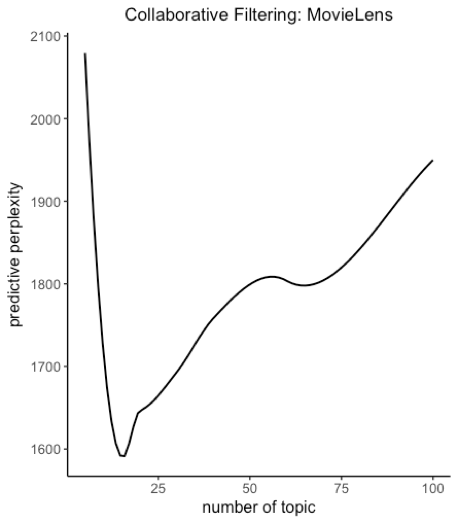
\includegraphics[scale=0.8]{cf_para_tune.png}
\centering
\end{figure}


we can see that the model with 15 topics predict the held-out movie best. Thus, we will use all data in training users to train the final model with 15 topics and check for performance on the testing users.

\subsection{Model Evaluation}
\label{sec:length}
Collaborative Filtering evaluation metric varies according to the goal of the tasks like whether you want to recommend the right items or annotate the message in the context. In our case, we will concentrate on finding the right items. One of effective metrics to evaluate recommendation system of this goal is to see the recall rate of this recommendation system versus the number of recommended movies. More precisely, we held out small part of the movies(1/5 in our case), and then we present user with M movies ranked by the probability they may exist in ones? profiles and evaluate based on which of these movies were actually in each users? profiles. The definition of recall rate can be defined as following:

\begin{displaymath}
recall\textrm{-}rate(M)=  \frac{M_{user\ likes} }{M_{held-out}}
\end{displaymath}

where $M_{user\ likes}$ is the the number of movies user likes and $M_{held-out}$ is the number of movies we held out for this user. The recommendation system recall rate will be the arithmetic average of recall rates or all users.

A Higher recall rate with lower M will be a better system. Besides, We also add a simple method using cosine to calculate the similarity between users to recommend them similar movies. We will take it as a baseline method to see how our LDA does in terms of the collaborative filtering. And the result is as Figure below.

\begin{figure}[h]
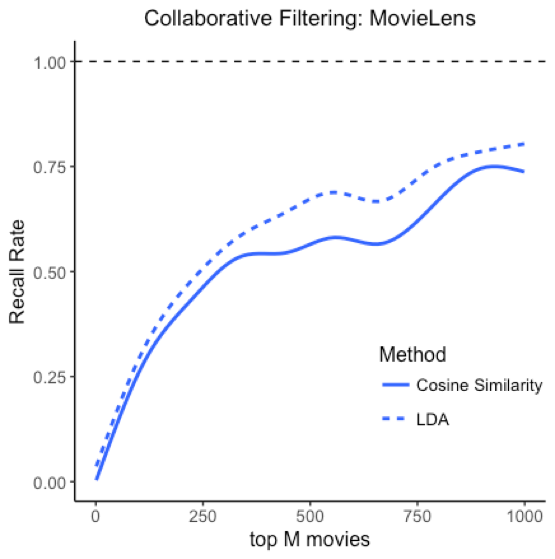
\includegraphics[scale=0.8]{cf_model_com.png}
\centering
\end{figure}

We can see that LDA does quite a good job and run much faster when the vocabulary is large compared with this traditional method, which needs to compute a large matrix. So LDA performs great in CF task when vocabulary is quite large compared with documents.

\section*{Acknowledgments}

% include your own bib file like this:
%\bibliographystyle{acl}
%\bibliography{acl2017}
\bibliography{acl2017}
\bibliographystyle{acl_natbib}

\appendix

\section{Supplemental Material}
\label{sec:supplemental}
ACL 2017 also encourages the submission of supplementary material
to report preprocessing decisions, model parameters, and other details
necessary for the replication of the experiments reported in the 
paper. Seemingly small preprocessing decisions can sometimes make
a large difference in performance, so it is crucial to record such
decisions to precisely characterize state-of-the-art methods.

Nonetheless, supplementary material should be supplementary (rather
than central) to the paper. {\bf Submissions that misuse the supplementary 
material may be rejected without review.}
Essentially, supplementary material may include explanations or details
of proofs or derivations that do not fit into the paper, lists of
features or feature templates, sample inputs and outputs for a system,
pseudo-code or source code, and data. (Source code and data should
be separate uploads, rather than part of the paper).

The paper should not rely on the supplementary material: while the paper
may refer to and cite the supplementary material and the supplementary material will be available to the
reviewers, they will not be asked to review the
supplementary material.

Appendices ({\em i.e.} supplementary material in the form of proofs, tables,
or pseudo-code) should come after the references, as shown here. Use
\verb|\appendix| before any appendix section to switch the section
numbering over to letters.

\section{Multiple Appendices}
\dots can be gotten by using more than one section. We hope you won't
need that.

\end{document}
